\documentclass[a4paper,12pt]{article}
\usepackage[tikz]{newlistok}
\usetikzlibrary{matrix}

%\documentstyle[11pt, russcorr, listok]{article}
\renewcommand{\spacer}{\vspace{1.8pt}}

%\УвеличитьШирину{1.1truecm}
\УвеличитьВысоту{1.5truecm}
%\hoffset=-2.5truecm
%\voffset=-27.3truemm
%\documentstyle[11pt, russcorr, ll]{article}

\pagestyle{empty}

\Заголовок{Перестановки: чётность}
\Подзаголовок{}
\НомерЛистка{49}
\ДатаЛистка{22.04.2020 -- 29.04.2020}
\Оценки{14/11/8}

\begin{document}


\СоздатьЗаголовок



\опр
\emph{Беспорядок} или \emph{инверсия} в перестановке $\alpha$
--- это такая пара $(i,j)$, что $i<j$ и $\alpha(i)>\alpha(j)$.
Перестановка называется \emph{чётной}, если число инверсий в ней
чётно, и \emph{нечётной} в противном случае.
Говорят также, что {\em знак} чётной перестановки равен $1$, а знак нечётной перестановки равен $-1$.
%Множество всех чётных перестановок из $S_n$ обозначается $A_n$ и называется \emph{знакопеременной группой}.
\копр


\пзадача
\вСтрочку
\пункт
Какие перестановки в $S_3$ чётные?\\
%\кзадача
%\задача
\пункт
Сколько инверсий у перестановки
$
\displaystyle
\begin{pmatrix}
1&2&\dots&n-1&n\\n&n-1&\dots&2&1
\end{pmatrix}
$?
\кзадача



\задача[Правило ниточек] Чтобы увидеть число инверсий геометрически, на картинке, можно поступить двумя способами. Первый: в таблице, отвечающей перестановке $\alpha$, соединим нитями одинаковые элементы (картинка слева). Второй: нарисуем таблицу с двумя одинаковыми верхними строками --- 1, 2, \ldots, $n$, --- и каждый элемент $i$ верхней строки соединим нитью с элементом $\alpha(i)$ во второй строке (картинка справа).\\
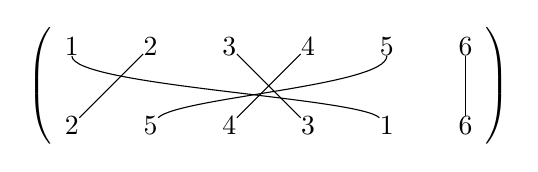
\begin{tikzpicture}%\usetikzlibrary{matrix}
\matrix [matrix of math nodes, column sep={1cm,between origins}, row sep={1cm,between origins},nodes={inner sep=0mm},
left delimiter=(,right delimiter=)]
{
|(A1)| 1 & |(A2)| 2 & |(A3)| 3 & |(A4)| 4 & |(A5)| 5 & |(A6)| 6 \\
|(B1)| 2 & |(B2)| 5 & |(B3)| 4 & |(B4)| 3 & |(B5)| 1 & |(B6)| 6 \\
};
\draw (A1) .. controls +(-90:5mm) and +(135:5mm) .. (B5);
\draw (A2) to (B1);
\draw (A3) to (B4);
\draw (A4) to (B3);
\draw (A5) .. controls +(-90:5mm) and +(45:5mm) ..  (B2);
\draw (A6) to (B6);
\end{tikzpicture}
\qquad
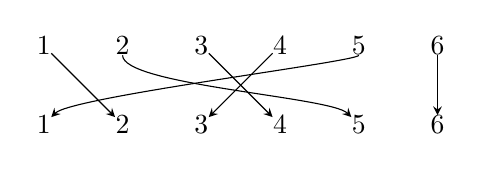
\begin{tikzpicture}[>=stealth,->]%\usetikzlibrary{matrix}
\matrix [matrix of math nodes, column sep={1cm,between origins}, row sep={1cm,between origins},nodes={inner sep=0mm}]
{
|(A1)| 1 & |(A2)| 2 & |(A3)| 3 & |(A4)| 4 & |(A5)| 5 & |(A6)| 6 \\
|(B1)| 1 & |(B2)| 2 & |(B3)| 3 & |(B4)| 4 & |(B5)| 5 & |(B6)| 6 \\
};
\draw (A1) to (B2);
\draw (A2) .. controls +(-90:5mm) and +(135:5mm) ..  (B5);
\draw (A3) to (B4);
\draw (A4) to (B3);
\draw (A5) .. controls +(-90:2mm) and +(45:5mm) ..  (B1);
\draw (A6) to (B6);
\end{tikzpicture}\\
\пункт Как увидеть количество инверсий на этой картинке  (можно дать ответ для одного способа)?\\
\ппункт Сделайте это для $(2\ 3\ 4)$ и $(14)(23)$ из $S_4$.\\
\ппункт Изменится ли чётность числа инверсий, если в нижней строке таблицы поменять два элемента местами?
\кзадача

\пзадача
Найдите число инверсий перестановки $\alpha^{-1}$, зная число инверсий перестановки $\alpha$.
\кзадача

\ввпзадача
\пункт Докажите, что любая транспозиция --- нечётная перестановка;\\
\пункт Докажите, что умножение на транспозицию (справа) меняет чётность перестановки;\\
\пункт Докажите, что произведение двух перестановок одной чётности ---
чётная перестановка, а~произведение двух перестановок разной
чётности --- нечётная (знаки перемножаются!).
\кзадача

\пзадача
Пусть $\alpha$ --- произвольная перестановка. Как связаны наименьшее число транспозиций в разложении $\alpha$ на элементарные транспозиции и число инверсий у $\alpha$?
\кзадача

\пзадача
Докажите, что чётность цикла зависит только от его длины. Как?
\кзадача


\пзадача
Сколько всего чётных перестановок в $S_n$? (Их множество обозначается $A_n$.)
\кзадача



\сзадача
В игре Сэма Лойда <<пятнашки>> поменяли квадраты с числами $14$ и $15$ местами. Можно ли из этой позиции по правилам игры получить исходную?
\кзадача

\сзадача
Для прохождения теста тысячу мудрецов выстраивают в колонну. Из колпаков с  номерами от 1 до 1001 один прячут, а остальные в случайном порядке надевают на мудрецов. Каждый видит только номера на колпаках всех впереди стоящих. Далее мудрецы по порядку от заднего к переднему называют вслух целые числа. Каждое число должно быть от 1 до 1001, причем нельзя называть то, что уже было сказано. Результат теста --- число мудрецов, назвавших номер своего колпака.  Мудрецы заранее знали условия теста и могли договориться, как действовать. Могут ли они гарантировать результат
\пункт  более 500;
%\пункт не менее 997?
\пункт не менее 999?
\кзадача


% \сзадача
% \пункт
% Почему задача Ллойда об игре в 15 неразрешима?
% \пункт
% Двудольный граф правильно раскрашен в 2 цвета.
% В каждой его вершине записано по числу (числа~разные).
% За ход можно менять местами любые 2 числа, соедин\"енные
% ребром. Может ли после нескольких ходов возникнуть ситуация,
% оказаться, что 2 числа одного цвета поменялись местами,
% а остальные числа на своих местах?
% \кзадача

% \сзадача
% У отца было 7 дочерей. Всякий раз, когда одна выходила замуж,
% каждая е\"е старшая сестра, оставшаяся в невестах,
% жаловалась отцу, что нарушен обычай выходить замуж
% по старшинству. После того, как вышла замуж последняя дочь,
% оказалось, что отец услышал всего 7 жалоб.
% В каком порядке дочери могли выходить замуж
% (приведите пример)? Сколько всего таких порядков?
% \кзадача
%

\пзадача Пусть $n\geq3$. Докажите, что $A_n$ --- это в точности множество перестановок из $S_n$, которые можно разложить в произведение циклов длины $3$ (повторения разрешаются).
\кзадача

\пзадача
Постройте такое соответствие между элементами $A_4$ и вращениями пространства, переводящими правильный тетраэдр в себя, что композиции перестановок  соответствует композиция соответствующих вращений.
\кзадача



% \сзадача Для каких $k$ в $S_n$ существует перестановка, у которой
% ровно $k$ инверсий?
% \кзадача

% \задача
% В каждой клетке таблицы $2\times n$ стоит одно из целых чисел от 1 до $n$,
% прич\"ем в каждой строке стоят разные числа, и
% в каждом столбце стоят разные числа. Сколько таких таблиц?
% \кзадача


% \сзадача
% В таблице $n$ строк и $m$ столбцов.
% \выд{Горизонтальный ход} --- это любая
% перестановка элементов таблицы, при которой
% каждый элемент остается в той же строке, что и до перестановки.
% Аналогично определяется \выд{вертикальный ход}. За какое наименьшее
% число %таких
% горизонтальных и вертикальных
% ходов всегда удастся получить любую перестановку элементов
% таблицы?
% \кзадача
%

% \задача
% Найдите в $S_n$ перестановку с максимальным возможным числом инверсий.
% \кзадача
%
% \сзадача
% Сколько всего в $S_n$ имеется циклов длины $n$ с наименьшим числом инверсий?
% \кзадача
%
%



\сзадача
% \пункт Перестановке $\alpha$ сопоставим набор чисел $a_1,a_2,\ldots,a_{n-1}$, где $a_i$ -- число пар $i<j$, таких что $\alpha(i)>\alpha(j)$. Очевидно, что $0\leqslant a_i\leqslant n{-}i$. Докажите, что набор чисел $a_1,a_2,\ldots,a_{n-1}$, полученный таким образом, однозначно определяет перестановку, а также любой набор, удовлетворяющий выписанным неравенствам, получается из некоторой перестановки указанным способом.\\
% \пункт Покажите, что любая перестановка однозначно представляется в виде $$(1{+}a_1\ \ldots\ 2\ 1)(2+a_2\ \ldots\ 3\ 2)\ldots(n{-}1+a_{n-1}\ \ldots\ n\ n{-}1), \qquad \text{где}\ 0\leqslant a_i\leqslant n{-}i.$$
% \noindent
%\пункт
Пусть $s_l$ -- количество перестановок с числом инверсий $l$. Покажите, что
$$1+s_1x+s_2x^2+s_3x^3+\ldots=(1+x)(1+x+x^2)\ldots(1+x+\ldots+x^{n-1}).$$
\кзадача



\ЛичныйКондуит{0mm}{5mm}
%\GenXMLW


\end{document}


\опр
Две перестановки $\alpha$ и $\beta$ {\em сопряжены}, если существует такая перестановка $\gamma$, что $\alpha=\gamma\beta\gamma^{-1}$.
\копр

\задача Докажите, что \пункт порядки у любых двух сопряжённых перестановок совпадают;
\пункт две перестановки сопряжены, если и только если наборы длин циклов в их разложении на непересекающиеся циклы совпадают.
\кзадача

\задача
Верно ли, что перестановки с одинаковым числом инверсий сопряжены?
\кзадача

\задача
Найдите хотя бы одну перестановку $x$, такую что $x^2=\alpha$, где $\alpha$ -- перестановка.
\кзадача
